%!TEX program = xelatex
% 完整编译方法 1 pdflatex -> bibtex -> pdflatex -> pdflatex
% 完整编译方法 2: xelatex -> bibtex -> xelatex -> xelatex
\documentclass[lang=cn,11pt]{elegantpaper}

\title{基于Hadoop MapReduce并行计算框架的邮件自动分类}
\author{曹佳涵 $\quad$ 白家杨 $\quad$ 刘笑今}

\institute{2019st04小组}

% 不需要版本信息,直接注释即可
\version{}
% 不需要时间信息的话,需要把 \today 删除。
\date{}


% 如果想修改参考文献样式,请把这行注释掉
\usepackage[authoryear]{gbt7714}  % 国标

\begin{document}

\maketitle

\begin{abstract}
\noindent 本实验的目标是通过 MapReduce 编程来实现邮件的自动分类,通过本课程设计的学习,可以体会如何使用 MapReduce 完成一个综合性的数据挖掘任务,包括全流程的数据预处理、样本分类、样本预测等。我们使用Hadoop MapReduce并行计算框架对原始邮件文本进行特征选择、特征向量权重计算、文本分类和样本预测任务,从而搭建起一个完整的文本分类处理流程。我们采用了不同的特征提取方法和分类算法并进行比较和分析。此外,我们使用Spark同样完成了实验。
\keywords{邮件分类,并行计算,MapReduce,Spark}
\end{abstract}

\section{引入}



此模板是基于 \LaTeX{} 的标准文类 article设计,也即意味着你可以把 article 文类的选项传递给本模板,比如 \lstinline{a4paper, 10pt} 等等(推荐使用 \lstinline{11pt})。本模板支持 \lstinline{PDFLaTeX} 和 \lstinline{XeLaTeX}\footnote{中文字体均使用 \lstinline{ctex} 包设置。} 两种编译方式。

数学字体的效果如下:

\begin{equation}
(a+3b)^{n} = \sum_{k=0}^{n} C_{n}^{k} a^{n-k} (3b)^k\label{eq:binom}
\end{equation}
      
\subsection{全局选项}
我在这个模板中定义了一个语言选项 \lstinline{lang},可以选择英文模式 \lstinline{lang=en}(默认)或者中文模式 \lstinline{lang=cn}。当选择中文模式时,图表的标题引导词以及参考文献,定理引导词等信息会变成中文。你可以通过下面两种方式来选择语言模式:

\begin{lstlisting}
\documentclass[lang=cn]{elegantpaper} % or
\documentclass{cn}{elegantpaper} 
\end{lstlisting}


\subsection{自定义命令}
在此模板中,并没有修改任何默认的命令或者环境,所以,你可以在此模板使用原来的命令和环境。另外,我自定义了 3 个命令:

\begin{enumerate}
	\item \lstinline{\email}:创建邮箱地址的链接;
	\item \lstinline{\figref}:用法和 \lstinline{\ref} 类似,但是会在插图的标题前添加 <\textbf{图 n}> ;
	\item \lstinline{\tabref}:用法和 \lstinline{\ref} 类似,但是会在表格的标题前添加 <\textbf{表 n}>;
	\item \lstinline{\keywords}:为摘要环境添加关键词。
\end{enumerate}

\subsection{列表环境}
你可以使用列表环境(\lstinline{itemize}、\lstinline{enumerate}、\lstinline{description}),示例如下:\\[2ex]
\begin{minipage}[c]{0.59\linewidth}
\begin{lstlisting}
\begin{itemize}
   \item Routing and resource discovery;
   \item Resilient and scalable networks; 
   \item Distributed storage and search.
\end{itemize}
\end{lstlisting}
\end{minipage}
\begin{minipage}[c]{0.4\linewidth}
\begin{itemize}
   \item Routing and resource discovery;
   \item Resilient and scalable networks;
   \item Distributed storage and search.
\end{itemize}
\end{minipage}




\subsection{插图}
插图的命令和以前一样,也是使用 \lstinline{figure} 环境。\figref{fig:scatter} 显示了插图的效果。你可以把你的图放到当前工作目录的如下子目录下 (\lstinline{./image/}, \lstinline{./img/}, \lstinline{./figure/}, \lstinline{./fig/})。


\begin{lstlisting}
\begin{figure}[htbp]
	\centering
	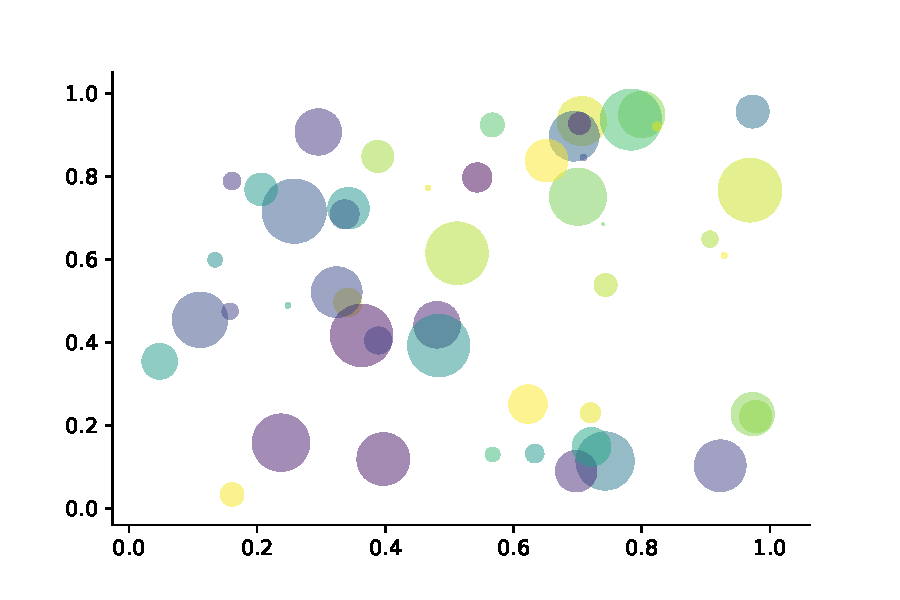
\includegraphics[width=0.6\textwidth]{scatter.pdf}
	\caption{Scatter Plot Example \label{fig:scatter}}
\end{figure}
\end{lstlisting}
\begin{figure}[htbp]
	\centering
	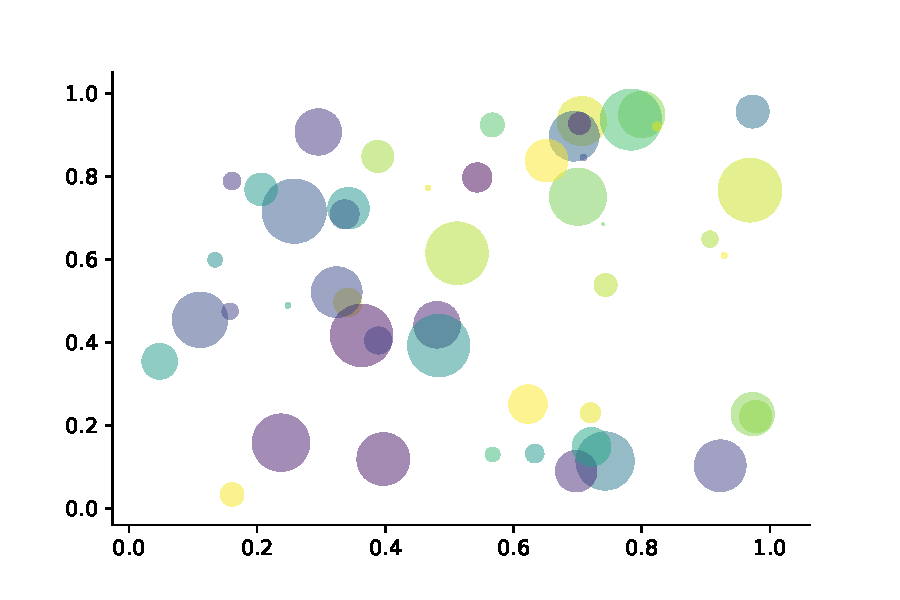
\includegraphics[width=0.6\textwidth]{scatter.pdf}
	\caption{Scatter Plot Example \label{fig:scatter}}
\end{figure}

\subsection{表格}
我强烈建议你使用 \lstinline{booktabs} 宏包,这个宏包有三个命令 \lstinline{\toprule}、\lstinline{\midrule} 和 \lstinline{\bottomrule} 能方便你制作三线表。\tabref{tab:reg} 是一个示例:

\begin{lstlisting}
\begin{table}[htbp]
  \small
  \centering
  \caption{Auto MPG and Price \label{tab:reg}}
    \begin{tabular}{lcc}
    \toprule
                    &       (1)         &        (2)      \\
    \midrule
    mpg             &    -238.90***     &      -49.51     \\
                    &     (53.08)       &      (86.16)    \\
    weight          &                   &      1.75***    \\
                    &                   &      (0.641)    \\
    constant        &     11,253***     &       1,946     \\
                    &     (1,171)       &      (3,597)    \\
    obs             &        74         &         74      \\
    $R^2$           &      0.220        &       0.293     \\
    \bottomrule
    \multicolumn{3}{l}{\scriptsize Standard errors in parentheses} \\
    \multicolumn{3}{l}{\scriptsize *** p<0.01, ** p<0.05, * p<0.1} \\
    \end{tabular}%
\end{table}%
\end{lstlisting}
\begin{table}[htbp]
  \small
  \centering
  \caption{Auto MPG and Price \label{tab:reg}}
    \begin{tabular}{lcc}
    \toprule
                    &       (1)         &        (2)      \\
    \midrule
    mpg             &    -238.90***     &      -49.51     \\
                    &     (53.08)       &      (86.16)    \\
    weight          &                   &      1.75***    \\
                    &                   &      (0.641)    \\
    constant        &     11,253***     &       1,946     \\
                    &     (1,171)       &      (3,597)   \\
    obs             &        74         &         74     \\
    $R^2$           &      0.220        &       0.293    \\
    \bottomrule
    \multicolumn{3}{l}{\scriptsize Standard errors in parentheses} \\
    \multicolumn{3}{l}{\scriptsize *** p<0.01, ** p<0.05, * p<0.1} \\
    \end{tabular}%
\end{table}%



\subsection{参考文献}
你可以在谷歌学术,Mendeley,Endnote 中获得文献条目(bib item),然后把它们添加到 \lstinline{wpref.bib} 中。在文中引用的时候,引用它们的键值(bib key)即可。注意需要在编译的过程中添加 Bib\TeX{} 编译。如果你想在参考文献中添加未引用的文献(部分或者全部),可以使用

\begin{lstlisting}
\nocite{EINAV2010, Havrylchyk2018} % add the two reference.
\nocite{*}   % add all the reference in the bib file.
\end{lstlisting}

如果你想修改参考文献的样式(比如改为 \lstinline{aer}),你可以在导言区将下面代码注释掉。
\begin{lstlisting}
\usepackage[authoryear]{gbt7714}
\end{lstlisting}

并且文档末尾添加

\begin{lstlisting}
\bibliographystyle{aer}
\end{lstlisting}

\section{数据分析}
这是一个有监督的多分类问题。对于训练数据全集,经过分析,共有20个类别,它们编号,名称,以及包含的邮件文本个数为:\par
\begin{table}[!htbp]
  \small
  \centering
  \caption{Auto MPG and Price \label{tab:reg}}
    \begin{tabular}{lcc|lcc}
    \toprule
    类别编号  &   类别名称  &   包含邮件文本个数  &   类别编号  & 类别名称  & 包含邮件文本个数  \\
    \hline
    1 & sci.electronics & 1000            & 11 & rec.sport.baseball & 1000 \\
    2 & comp.windows.x & 1000             & 12 & rec.autos & 1000 \\
    3 & talk.politics.mideast & 1000      & 13 & talk.politics.misc & 1000 \\
    4 & comp.os.ms-windows.misc & 1000    & 14 & talk.politics.guns & 1000 \\
    5 & rec.sport.hockey & 1000           & 15 & comp.graphics & 1000 \\
    6 & sci.crypt & 1000                  & 16 & soc.religion.christian & 997 \\
    7 & comp.sys.mac.hardware & 1000      & 17 & rec.motorcycles & 1000 \\
    8 & sci.space & 1000                  & 18 & misc.forsale & 1000 \\
    9 & talk.religion.misc & 1000         & 19 & sci.med & 1000 \\
    10 & comp.sys.ibm.pc.hardware & 1000  & 20 & alt.atheism & 1000 \\
    \bottomrule
    \end{tabular}%
\end{table}%\
可以看到,训练样本全集共有20个类别,训练样本总数为19997个,每个类别下训练样本的数量是平衡的,几乎都是1000个,因此在进行训练时,不需要考虑类别不平衡问题。


\section{MapReduce处理流程}
\subsection{特征选择}
本任务的主要工作是对原始的邮件文本中进行特征选择,选择出能够表征邮件主题的特征词,为后续的文本分类做准备。\par
对于输入的未分词的邮件训练样本全集和停词表,我们需要输出全局邮件文本特征,并对它们进行相应的编号,此外,对于训练数据集的目录,将目录名(即文本类别)转换为相应的类别序号。\par
对于该任务,我们采用了两种计算方法,分别为半并行化和并行化计算方法。
\subsubsection{半并行化计算方法}
半并行化计算方法是指将该任务划分为两个步骤,第一步读取训练样本全集和停词表,生成干净文本;第二步读取干净文本,生成全局邮件特征集。\par
第一步的主要思路是顺序执行,首先读取20\_newsgroup文件夹下的子文件夹,将子文件夹名(即类别名)转化为类编号并进行存储。将 Lucene 的 Standard Analyzer 分词器作为基类,输入停词表,自定义自己的带有停词表功能的停词器,然后顺序依次读取每个子文件夹下的所有文件,使用自定义的停词器对文本进行分词,并将分词结果储存在目标文件中,我们将分词后的文本称为干净文本,生成干净文本的过程是顺序执行,非并行化的。为了后续处理的方便性,我们修改输出文件的格式为:filename-classNum,filename为原文件的文件名,classNum为它所属的类别的编号,两者用分隔符 '-' 隔开。\par
\begin{algorithm}[!htb]
  \caption{特征选择半并行化算法:第一步}
  \label{alg:Framwork}
  \begin{algorithmic}[1]
    \Require
    邮件训练样本全集 $U$,停词表 $S$
    \Ensure
    用停词表分割后的干净文本
    \State 初始化类别名-类别编号对应表 classMap
    \State 初始化停词器 stopAnalyzer=StopAnalyzer($S$)
      \For{each 文本 $u$ in $U$}
      \State 新文本 $u^\prime$ = stopAnalyzer(u)
      \State 通过类别名-编号对应表查找文本$u$的文件名filename对应的类别编号num=classMap($u$)
      \State 在目标目录下创建filename-num文件,并将新文本$u^\prime$的内容写入该文件。
   \EndFor
  \end{algorithmic}
\end{algorithm}
第二步从干净文本中提取全局邮件文本特征集的过程是并行化的,使用MapReduce并行计算框架,在Map阶段读取干净文本,对于每一个单词word,发射(word,1)键值对。在Reduce阶段,设置一个全局缓存变量$n$,为每个单词维护一个编号,并将每个单词和相应的编号输出到全局邮件特征集中。\par
\begin{algorithm}[!htb]
  \caption{特征选择半并行化算法:第二步}
  \label{alg:Framwork}
  \begin{algorithmic}[1]
    \Require
    干净文本 $U^\prime$
    \Ensure
    \State \textbf{Map阶段}:
    \Function {map}{$filename$, $text$}
      \For{each word $w$ in $text$}
        \State Emit($w$,$1$)
      \EndFor
    \EndFunction
    \State \textbf{Reduce阶段}:
    \Function {reduce}{$word$, $value$}
      \State 全局缓存变量$num=num+1$
      \State 将$word$和$num$写入到全局邮件文本特征集中
      \State Emit($word$,$value$)
    \EndFunction
  \end{algorithmic}
\end{algorithm}

\subsubsection{并行化计算方法}
非并行化顺序执行,缺点也显而易见:计算速度慢,效率低,因此我们设计了并行化的计算方法,利用 MapReduce 计算框架,很好地并行处理大量的训练文本,极大地加快了处理速度。\par
在Map阶段读取原文本,利用停词器将其分词后输出到目标目录下,同时对于每一个单词,发射(word,filename-classNum)键值对。值得注意的是,因为停词表是所有Mapper都需要各自初始化的,因此将其初始化放在Map阶段的setup过程中,首先将停词表文件路径存在DistributedCache中,然后在setup过程中读取该路径并利用其初始化停词器,在map过程中使用该停词器。\par
在Reduce阶段,设置一个全局缓存变量$n$,用来表示每一个单词的唯一标号。输入为(word, value)。由于在Reduce阶段,已经将相同key的键值对都整合到了一起,因此读取的word值是唯一不重复的,只需要利用全局变量$n$为每一个单词分配相应的标号,并将单词和编号输出到目标文件中即可。\par
\begin{algorithm}[!htb]  
  \caption{特征选择并行化算法}  
  \label{alg:Framwork}
  \begin{algorithmic}[1]
    \Require
    邮件训练样本全集 $U$,停词表 $S$
    \Ensure 
    用停词表分割后的干净文本,全局邮件文本特征集
    \State 初始化类别名-类别编号对应表 classMap
    \State 将停词表$S$ 存入DistributedCache中
    \State \textbf{Map阶段}:
    \Function {setup}{}
    \State 从DistributedCache中读取停词表$S$
    \State 初始化停词器 stopAnalyzer=StopAnalyzer($S$)
    \EndFunction
    \Function {map}{$filename$, $text$}
      \State $text^\prime$ = stopAnalyzer($text$)
      \State 将$text^\prime$写入到目标干净文本中
      \For{each word $w$ in $text^\prime$}
        \State Emit($w$,$filename$)
      \EndFor
    \EndFunction
    \State \textbf{Reduce阶段}:
    \Function {reduce}{$word$, $value$}
      \State 全局缓存变量$num=num+1$
      \State 将$word$和$num$写入到全局邮件文本特征集中
      \State Emit($word$,$filename$)
    \EndFunction
  \end{algorithmic}
\end{algorithm}

\subsubsection{运行结果}
该任务的输出结果如下图所示:
\begin{figure}[!htbp]
	\centering
	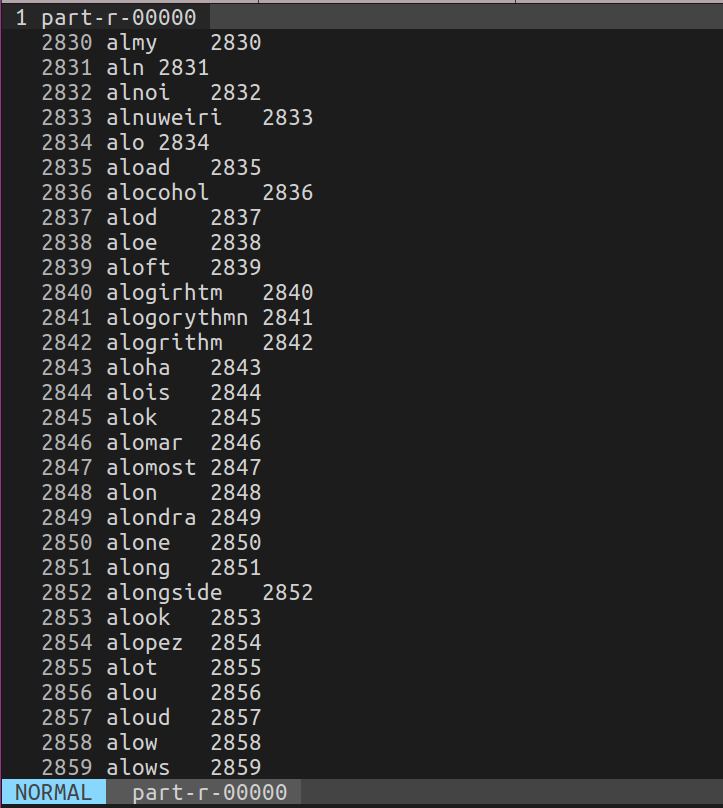
\includegraphics[width=0.6\textwidth]{feature-out.png}
	\caption{全局邮件文本特征 \label{fig:feature-out}}
\end{figure}

\subsection{特征向量权重计算}
本任务主要是基于任务一输出的特征词向量,计算出每个邮件样本的特征词权重,特征词权重用来刻画特征词在描述此文本内容时所起的重要程度。\par
目前流行的特征向量权重算法大多是通过构造评估函数,对特征集合中的每个特征进行评估,并对每个特征打分,这样每个词语都获得一个评估值,又称为权值。然后将所有特征按权值大小排序,提取预定数目的最优特征作为提取结果的特征子集。显然,对于这类型算法,决定文本特征提取效果的主要因素是评估函数的质量。\par
目前常见的特征向量权重算法有TF-IDF,词频方法(Word Frequency),文档频次方法(Document Frequency),互信息(Mutual Information),期望交叉熵(Expected Cross Entropy),x2统计量方法,文本证据权(The Weight of Evidence forText)等。在本任务中,我们采用TF-IDF算法。
\subsubsection{原理解释}
TF-IDF(term frequency–inverse document frequency)是一种用于资讯检索与资讯探勘的常用加权技术。TF-IDF是一种统计方法,用以评估一字词对于一个文件集或一个语料库中的其中一份文件的重要程度。字词的重要性随着它在文件中出现的次数成正比增加,但同时会随着它在语料库中出现的频率成反比下降。TF-IDF加权的各种形式常被搜寻引擎应用,作为文件与用户查询之间相关程度的度量或评级。\par
在一份给定的文件里,词频(term frequency,TF)指的是某一个给定的词语在该文件中出现的频率。这个数字是对词数(term count)的归一化,以防止它偏向长的文件。(同一个词语在长文件里可能会比短文件有更高的词数,而不管该词语重要与否。)对于在某一特定文件里的词语 $t_{i}$ 来说,它的重要性可表示为:\par
$$\mathrm{tf}_{i,j}=\frac{n_{i,j}}{\sum_{k}n_{k,j}}$$
以上式子中 $n_{i,j}$ 是该词$t_{i}$ 在文件$d_{j}$中的出现次数,而分母则是在文件$d_{j}$中所有字词的出现次数之和。\par
逆向文件频率(inverse document frequency,IDF)是一个词语普遍重要性的度量。某一特定词语的IDF,可以由总文件数目除以包含该词语之文件的数目,再将得到的商取对数得到:\par
$$\mathrm{idf_{i}} =  \log \frac{|D|}{|\{j: t_{i} \in d_{j}\}|}$$
其中 $|D|$是语料库中的文件总数,$|\{ j: t_{i} \in d_{j}\}|$是包含词语$t_{i}$的文件数目(即$n_{i,j} \neq 0$的文件数目)如果该词语不在语料库中,就会导致被除数为零,因此一般情况下使用$1 + |\{j : t_{i} \in d_{j}\}|$\par
将TF值和IDF值相乘,即获得最终的TF-IDF值。\par
$$\mathrm{tf{}idf_{i,j}} = \mathrm{tf_{i,j}} \times  \mathrm{idf_{i}}$$
某一特定文件内的高词语频率,以及该词语在整个文件集合中的低文件频率,可以产生出高权重的TF-IDF。因此,TF-IDF倾向于过滤掉常见的词语,保留重要的词语。

\subsection{Hadoop MapReduce 实现}
由于TF-IDF设计到TF和IDF两种不同指标的计算,所以所有计算难以直接在一个job中完成。我们通过分解,将其划分为三个Job,分别对应于计算的三个阶段:TF计算(TF-Job),IDF计算(IDF-Job)和TF、IDF相乘的整合阶段(Integrate-Job)。

\begin{figure}[htbp]
	\centering
	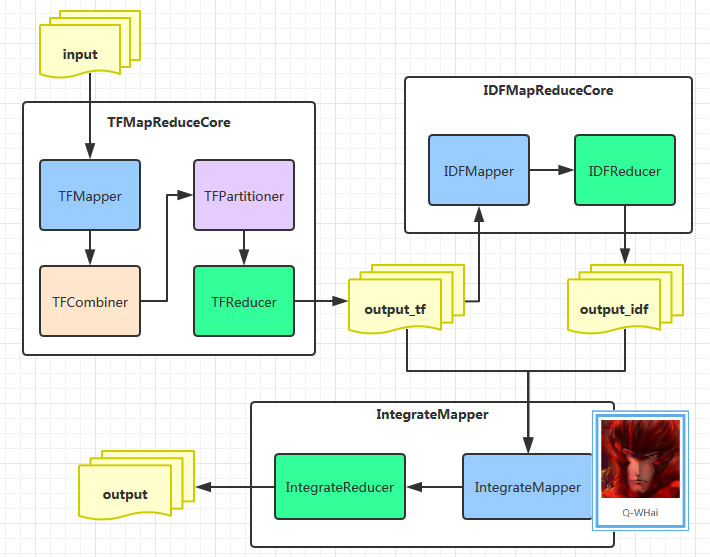
\includegraphics[width=0.6\textwidth]{tfidf_framework.png}
	\caption{TF-IDF算法框架 \label{fig:tfidf_framework}}
\end{figure}

\subsubsection{TF-Job}
在TF Job中,主要任务是统计每个文件所有单词个数以及每个单词的出现次数,并计算每个单词在每个文件中的出现比例。\par
在Map阶段,读取在上个任务中生成的干净文本,输入为(文件名filenanme-文本内容text)键值对,对于每一个单词word,发射(word:filename, 1)键值对,同时文本单词数量计数器count加一,当整个文本遍历完成后,发射(!:count)键值对。值得注意的是,我们还需要自定义Partitioner,因为我们希望传入Reducer的数据按文件名排序(即key中':'后面的字符串),所以在自定义Partitioner中需要分割key并取':'后面的filename作为划分和排序标准。\par
在Reduce阶段,输入为(xxx:filename, list[v1, v2, ...])键值对,此处xxx可能是单词word,也可能是标记符'!',当它是'!'时,value中存储的是该file中所有单词的数量,由于'!'是键盘上可输出的字符的ASCII码最小的字符,并且我们的自定义Partitioner使得来自相同文本(即filename相同)的键值对排列在一起并且传入同一个Reudcer,因此对于任意一个文本,所有来自它的键值对中(!:filename,value)是第一个被Reducer接收到的键值对,因此我们将其存储到全局缓存变量allWordCnt中;当它是word时,list[v1,v2,...]中存储的是该word在该file中的出现次数列表,将其相加即可获得该单词在该文本中的频数,此时全局缓存变量allWordCnt存储的是该文本中所有单词的数量,将二者相除即可得到该单词在该文本中的TF值,最后发射键值对(word:filename, tf)。\par
\begin{algorithm}[!htb]  
  \caption{TF-IDF算法: TF-Job}  
  \label{alg:Framwork}
  \begin{algorithmic}[1]
    \Require
    干净训练文本全集$D$
    \Ensure
    所有文本下所有单词的TF值
    \State \textbf{Map阶段}:
    \Function {setup}{}
    \State 初始化全局缓存变量 $n=0$
    \EndFunction
    \Function {map}{$filename$, $text$}
      \For{each word $w$ in $text$}
        \State Emit($w:filename$,$1$)
      \EndFor
    \EndFunction
    \State \textbf{Reduce阶段}:
    \Function {reduce}{$key$, $value=list[v_1,v_2,...]$}
    \If{$key$.beginWith('!')}
      \State 全局缓存变量 $n=value$
    \Else
      \State $sum=0$
      \For{each $v$ in $list[v_1,v_2,...]$}
        \State $sum = sum + v$
      \EndFor
      \State $tf = \frac{sum}{n}$
      \State Emit($key$, $tf$)
    \EndIf
    \EndFunction
  \end{algorithmic}
\end{algorithm}

\subsubsection{IDF-Job}
在IDF-Job中,需要计算两个值,一是文档数目,这个可以在Reducer外读取上下文信息来获得,另一个是包含某个单词的文件数目,由于TF-Job中已经输出(word:filename, tf)键值对,因此只需要读取TF-Job的输出,解析word和filename的对应关系,统计同一个包含同一个word的文件数目即可,这是一个典型的WordCount任务。\par
在Map阶段,从输入的(key, text)键值对的text字符串按':'分割,':'前面的子字符串即为单词word,发射键值对(word,1)。\par
在Reduce阶段,输入为(word, list[v1,v2,...]),只需要将list[v1,v2,...]累加起来,即为包含单词word的文档个数,利用公式$\mathrm{idf_{i}} =  \log \frac{|D|}{|\{j: t_{i} \in d_{j}\}|}$可以求得IDF值,最后发射键值对(word,idf)。\par
\begin{algorithm}[!htb]  
  \caption{TF-IDF算法: IDF-Job}  
  \label{alg:Framwork}
  \begin{algorithmic}[1]
    \Require
    TF-Job的输出文本$T$
    \Ensure
    所有单词的IDF值
    \State \textbf{Map阶段}:
    \Function {map}{$filename$, $text$}
      \State $word=$ split($text$, '!')[0]
    \EndFunction
    \State \textbf{Reduce阶段}:
    \Function {reduce}{$key$, $value=list[v_1,v_2,...]$}
      \State $sum=0$
      \For{each $v$ in $list[v_1,v_2,...]$}
        \State $sum = sum + v$
      \EndFor
      \State $n=$ getProfileNum()
      \State $idf = \log\frac{n}{sum}$
      \State Emit($key$, $idf$)
    \EndFunction
  \end{algorithmic}
\end{algorithm}

\subsubsection{Integrate-Job}
在Integrate-Job中,由于TF-Job和IDF-Job的输出文件格式不统一,因此主要任务是读取两个不同格式的文件,并将TF值和IDF值解析出来,最后相乘得到TF-IDF值。\par
TF-Job的输出文件格式为:
  \begin{lstlisting}[language={[ANSI]C},numbers=left,numberstyle=\tiny,%frame=shadowbox,  
     rulesepcolor=\color{red!20!green!20!blue!20},  
     keywordstyle=\color{blue!70!black},  
     commentstyle=\color{blue!90!},  
     basicstyle=\ttfamily]  
    word1:filename1   tf11
    word2:filename1   tf21
    word1:filename2   tf12
    ...
  \end{lstlisting}\par
IDF-Job的输出文件格式为:
\begin{lstlisting}[language={[ANSI]C},numbers=left,numberstyle=\tiny,%frame=shadowbox,  
  rulesepcolor=\color{red!20!green!20!blue!20},  
  keywordstyle=\color{blue!70!black},  
  commentstyle=\color{blue!90!},  
  basicstyle=\ttfamily]  
 word1  idf1
 word2  idf2
 ...
\end{lstlisting}\par
因此在处理时,在Map阶段,将读入的文本分割回原本的格式,发射(word:filename, tf)键值对或(word,idf)键值对。在Reduce阶段,对两种不同类型的key分开处理。此处利用了按key排序的特性,对于包含同一个word的key,一定是(word,idf)键值对先被读入,然后再读入(word,filename,idf)键值对,因此,先将idf值存入全局缓存变量中,然后将该idf和后续的每个属于该单词的不同文本的TF值相乘,即可获得最终每个单词每个文本的TF-IDF值。\par
\begin{algorithm}[htb]  
  \caption{TF-IDF算法: Integrate-Job}  
  \label{alg:Framwork}
  \begin{algorithmic}[1]
    \Require
    TF-Job的输出文本$T$,IDF-Job的输出文本$I$
    \Ensure
    所有单词所有文本的TF-IDF值
    \State \textbf{Map阶段}:
    \Function {map}{$filename$, $text$}
      \State $key^\prime=$ split($text$, '$\backslash$t')[0]
      \State $value^\prime=$ split($text$, '$\backslash$t')[1]
      \State Emit($key^\prime$,$value^\prime$)
    \EndFunction
    \State \textbf{Reduce阶段}:
    \Function {reduce}{$key$, $value$}
      \If{$key$.contains(':')}
        \State $tfidf$ = $value\times idf$
        \State Emit(key, tfidf)
      \Else
        \State 全局缓存变量 $idf=value$
      \EndIf
    \EndFunction
  \end{algorithmic}
\end{algorithm}

\subsection{运行结果}
通过将TF-IDF任务的输出格式整理后,最终的输出结果如下图所示:
\begin{figure}[htbp]
	\centering
	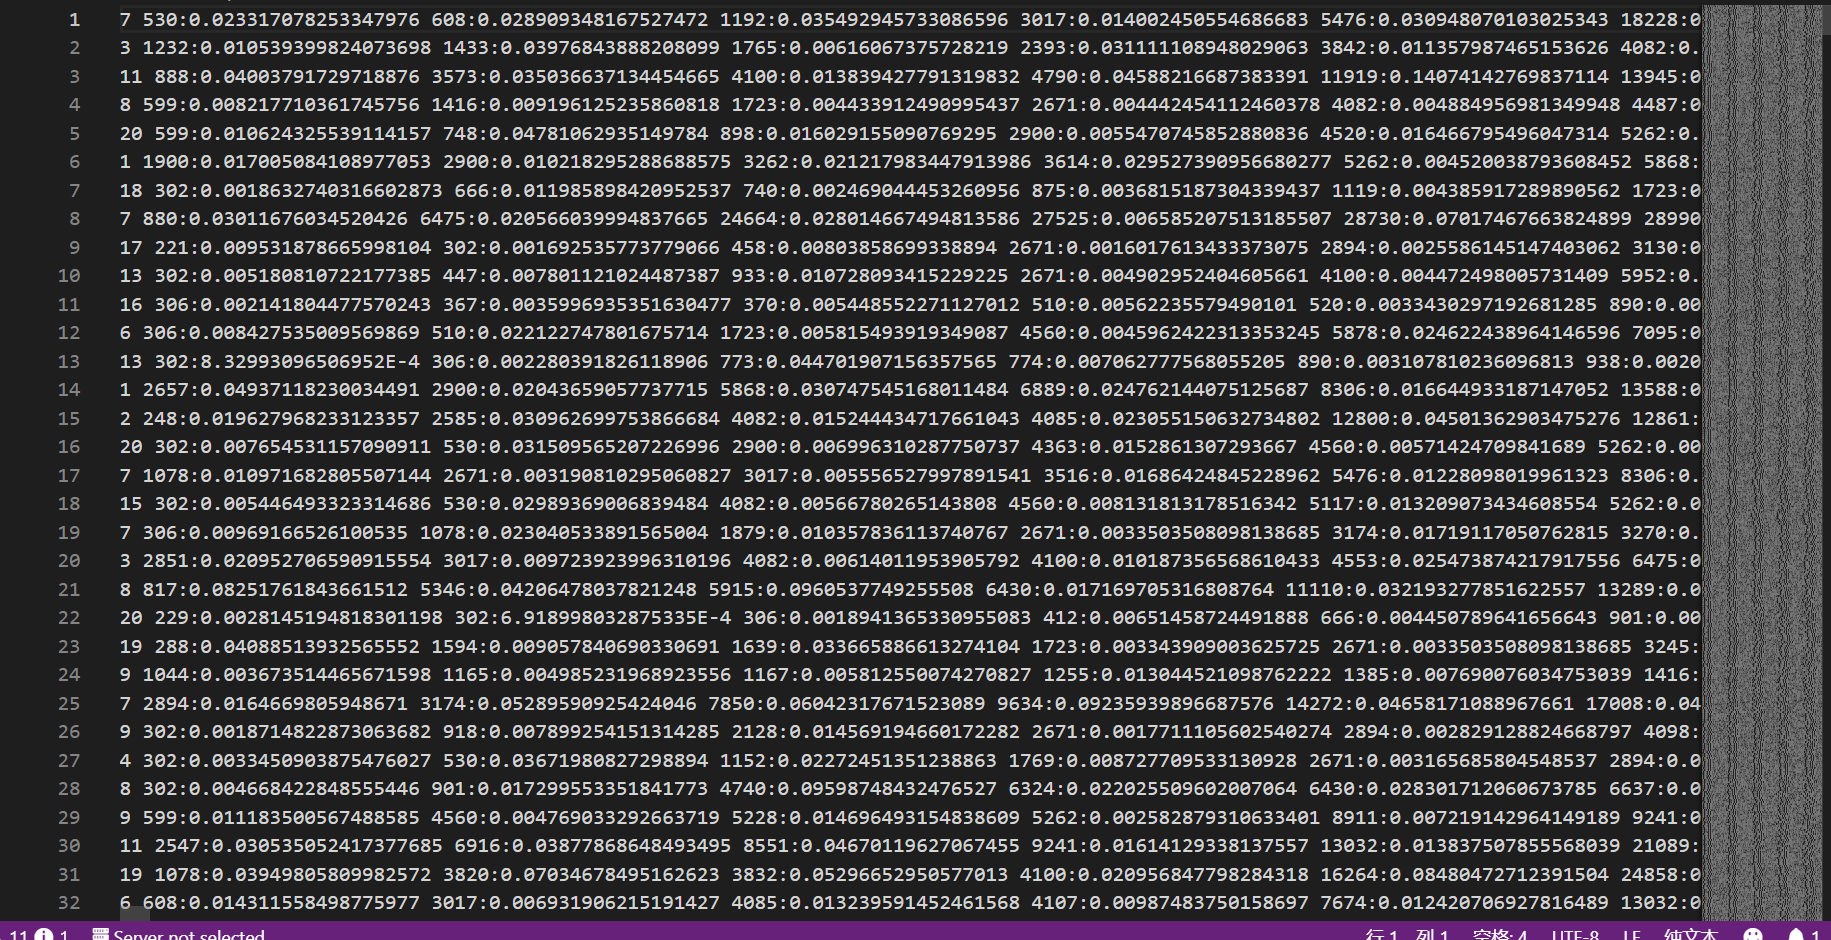
\includegraphics[width=0.6\textwidth]{tfidf.png}
	\caption{特征向量权重计算(TF-IDF) \label{fig:tfidf}}
\end{figure}

\subsection{朴素贝叶斯}
\subsubsection{原理推导}
朴素贝叶斯算法是生成模型中分类算法之一。所有朴素贝叶斯分类器都假设特定特征的值独立于给定类变量的任何其他特征的值。例如,如果水果是红色的,圆形的,直径约10厘米,则可以认为它是苹果。朴素贝叶斯分类器认为这些特征中的每一个都独立地贡献于该果实是苹果的概率,而不管任何可能的颜色,圆度和直径特征之间的相关性。
抽象来看,朴素贝叶斯是一个条件概率模型:给定一个要分类的问题实例,用向量表示 $ \mathbf {x} =(x_ {1} , \dots, x_ {n})$代表一些n个特征(自变量),它为这个实例分配概率$p(C_ {k} \mid x_ {1}, \dots, x_ {n})$其中$C_{k}$表示$K$个可能的类别中的一个 。
使用贝叶斯定理,条件概率可以分解为
$$p(C_ {k} \mid \mathbf {x})= {\frac {p(C_ {k})p (\mathbf {x} \mid C_ {k})} {p(\mathbf {x} )}}$$
“朴素”的条件独立假设发挥作用:假设所有特征都在$\mathbf {x}$是相互独立的,对类的条件$ C_ {k}$。在这个假设下,
$$p(x_ {i}\mid x_ {i+1},\dots,x_ {n},C_ {k})= p(x_ {i} \mid C_ {k})$$
因此,可以表示为
$$p(C_ {k} \mid x_ {1},\dots,x_ {n})= \frac{p(C_ {k})}{p(\mathbf {x})}\prod_ {i = 1}^{n} p(x_ {i} \mid C_ {k})$$
因此只要比较$p(C_ {k})\prod_ {i = 1}^{n} p(x_ {i} \mid C_ {k})$的值就可以判断类别。即为求下式
$$\hat{y} = {\underset {k \in \ {1,\dots,K}} {\operatorname {argmax}}} \ p(C_ {k})\prod_{i = 1} ^ {n} p(x_ {i} \mid C_ {k})$$
常用的有高斯朴素贝叶斯,伯努利朴素贝叶斯Bernoulli和多项式朴素贝叶斯Multinomial三种。
高斯朴素贝叶斯当处理连续数据时,典型的假设是与每个类相关联的连续值根据正态(或高斯)分布分布。
多项式朴素贝叶斯使用多项事件模型,样本(特征向量)表示多项式生成某些事件的频率 $(p_ {1},\dots,p_ {n})$其中 $p_i$是事件i发生的概率(或多类情况下的K个多项式)。在词袋模型中事件表示单个文档中单词的出现。
伯努利朴素贝叶斯:在多变量伯努利事件模型中,特征是描述输入的独立布尔值(二元变量)。
尽管朴素贝叶斯分类器具有朴素设计和明显过于简单的假设,但它在许多复杂的现实世界中仍然运行良好。综合比较表明,贝叶斯分类的表现优于其他方法,特别是在文本处理方面。
\subsubsection{Hadoop MapReduce实现}
词袋模型就是表示文本特征的一种方式。给定一篇文档,它会有很多特征,比如文档中每个单词出现的次数、某些单词出现的位置、单词的长度、单词出现的频率……而词袋模型只考虑一篇文档中单词出现的频率(次数),用每个单词出现的频率作为文档的特征(或者说用单词出现的频率来代表该文档)。利用词袋模型表示文本特征来进行朴素贝叶斯分类器的实现。
实际上就是求
$$\hat{y} = {\underset {k \in \ {1,\dots,K}} {\operatorname {argmax}}} \ p(C_ {k})\prod_{i = 1} ^ {n} p(w_ {i} \mid C_ {k})$$
其中$w_i$表示文档中的第i个单词。
由于每个概率值很小(比如0.0001)若干个很小的概率值直接相乘,得到的结果会越来越小。为了避免计算过程出现下溢,最终无法比较,引入对数函数Log,在 Log 空间中进行计算。然后得到如下公式
$$\hat{y} = {\underset {k \in \ {1,\dots,K}} {\operatorname {argmax}}} \ log \ p(C_ {k}) + \sum_{i = 1} ^ {n} log \ p(w_ {i} \mid C_ {k})$$
训练朴素贝叶斯的过程其实就是计算先验概率$p(C_k)​$和后半部分似然函数的过程。

\subsubsection{先验概率$p(c)$的计算}
$P(C_k)$的意思是:在所有的文档中,类别为$C_{k}$的文档出现的概率有多大。假设训练数据中一共有$N_{doc}$篇文档,只要数一下类别$C_{k}$的文档有多少个就能计算$P(C_k)$了,类别$C_{k}$的文档共有$N_k$篇,先验概率的计算公式如下:
$$p(C_k)=\frac{N_K}{N_{doc}}$$

\subsubsection{似然函数 $p(w_i|C_k)$ 的计算}
由于是用词袋模型表示一篇文档d,对于文档d中的每个单词$w_i$,找到训练数据集中所有类别为$C_{k}$的文档,数一数 单词$w_i$在这些文档(类别为$C_{k}$)中出现的次数:$count(w_{i},C_{k})$。
然后,再数一数训练数据集中类别为$C_{k}​$的文档一共有多少个单词
$$\sum_{w \in v}count(w, C_{k})$$
其中V是词库,即所有在文本中出现过的单词。(有些单词在词库中,但是不属于类别$C_{k}$,那么 $count(w, C_{k}) = 0​$
计算二者之间的比值,就是似然函数的值。似然函数计算公式如下:
$$p(w_ {i} \mid C_ {k})=\frac{count(w_i, C_k)}{\sum_{w \in v}count(w, C_{k})}$$
需要考虑特殊情况某一类的文档不包含某个词时,考虑add-one-smoothing,类似于拉普拉斯修正,其实就是将“出现次数加一”。此时似然函数变为:
$$p(w_ {i} \mid C_ {k})=\frac{count(w_i, C_k)+1}{\sum_{w \in v}(count(w, C_{k})+1)}=\frac{count(w_i, C_k)+1}{\sum_{w \in v}count(w, C_{k})+|V|}$$
其中$|V|$表示词库的单词数。
\subsubsection{Hadoop MapReduce的实现}
首先需要数据预处理,计算每个类对应的文件数便于接下来计算先验概率$p(c)$。用一个Job来实现这个功能。

在这个Job的Map阶段,输入的是前面经过处理的文件格式:每个样本是一个文件,文件名为“文件名-类编号”的格式。在Map阶段中利用split得到相应的文件名和类编号,输出键值对<类编号,文件名>

在Reduce阶段,用一个全局缓存变量Set来保存一个类编号的文件名,合并计算得到Set的元素个数就是类编号对应的文件数,最终输出键值对<类编号,文件数>到输出文件中。

算法伪代码如下。
\begin{algorithm}[!htb]
  \caption{预处理得到类与对应的文件数关系}
  \label{alg:Framwork}
  \begin{algorithmic}[1]
    \Require
    邮件训练样本全集 $U$
    \Ensure
    输出键值对<类编号,文件名>
    \State Map阶段:得到相应的文件名和类编号,输出键值对<类编号,文件名>
    \Function {map}{$key$, $text$}
      \For{each 单词 $w$ in $text$}
        \State 类名编号$classnum$ = getFileName($w$)).split("-")[1]
		 \State 文件名$filename$ = getFileName($w$)).split("-")[0]
        \State Emit($classnum$ , $filename$)
      \EndFor
   \EndFunction

  \State Reduce阶段:合并并输出<类编号,文件数量>到输出文件中
  \State 定义全局缓存变量 Map<String,int> $list$记录类编号对应文件数量
  
  \Function {reduce}{$key$, $values$}
    \State 定义全局缓存变量 Set<String> $files$
    \For{$value$ in $values$}
        \State $files$.add($value$)
    \EndFor
    \State $list$.put(($key$, $files$.size())
  \EndFunction
  \Function {cleanup}{}
    \For{($key$, $value$) in $list$}
        \State Emit($key$, $value$)
    \EndFor
  \EndFunction
  \end{algorithmic}
\end{algorithm}

最终得到的输出结果截图如下:
\begin{figure}[htbp]
	\centering
	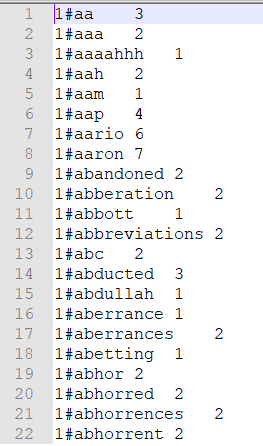
\includegraphics[width=0.4\textwidth]{BayesTrainResult.png}
	\caption{训练Job输出结果 \label{fig:BayesTrainResult}}
\end{figure}

在Hadoop MapReduce的实现中分成了两个Job来完成,分别是训练阶段的Job和预测阶段的Job。

在训练阶段的Job中实现的功能是对每个样本中的每个单词,输出键值对<类编号\#单词,单词出现的次数>。使用这种结构的好处是:可以通过Map映射方便找到每个单词在不同类中的出现次数。

在Map阶段中,利用FileSplit结构获得文件名,从文件名中就可以的获得单词所属的类别。用StringTokenizer划分出单词,对每个单词输出键值对<类编号\#单词, 1>

在Combine和Reduce阶段中,对读入的键值对<类编号\#单词,单词出现的次数>进行合并,最后输出即可。

第一个Job算法伪代码如下算法。

\begin{algorithm}[!htb]
  \caption{朴素贝叶斯训练阶段第一个Job}
  \label{alg:Framwork}
  \begin{algorithmic}[1]
    \Require
    邮件训练样本全集 $U$
    \Ensure
    输出训练结果文件,记录键值对<类编号\#单词,数量>
    \State Map阶段:分割每个单词并根据文件名获得类名编号,输出<类编号\#单词,数量>
    \Function {map}{$key$, $text$}
      \For{each 单词 $w$ in $text$}
        \State 类名编号$classnum$ = getClassNum(getFileName($w$))
        \State Emit($classnum$ + "\#" + $w$, 1)
      \EndFor
   \EndFunction

	\State Combine阶段:合并<类名\#单词,$num1$>、<类名\#单词,$num2$>为<类名\#单词,$num1+num2$>
  \State Reduce阶段:合并并输出<类名\#单词,数量>到输出文件中
  \Function {reduce}{$key$, $values$}
    \State $sum = 0$
    \For{$value$ in $values$}
        \State $sum += value$
    \EndFor
    \State Emit($key$, $sum$)
  \EndFunction
  \end{algorithmic}
\end{algorithm}

最终得到的输出结果截图如下:
\begin{figure}[htbp]
	\centering
	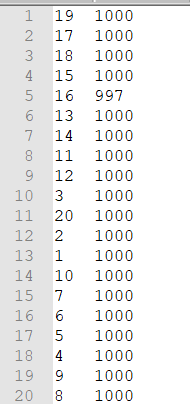
\includegraphics[width=0.4\textwidth]{GetClassNum.png}
	\caption{类编号与对应文件数 \label{fig:GetClassNum}}
\end{figure}

预测阶段Job实现根据样本数据,计算朴素贝叶斯方法下每个样本对应各个类的概率,比较得到最大概率对应的类别就是预测类别。

在Map的setup阶段中,先将训练阶段的键值对输出结果<类名\#单词,出现次数>保存到全局缓存变量Map结构体中,并计算得到每个类对应的单词总数,作为<类名,单词总数量>也加入到Map中。同时构建全局缓存变量Set结构体作为词库,将出现过的单词加入到Set中,Set中元素个数就是词库的大小。

在map阶段,对每个样本的每个单词$w_i$,计算对每个类$c$的似然函数的值$v=p(w|C_{k})=\frac{count(w_i, c)+1}{\sum_{w \in v}(count(w, C_{k})+1)}=\frac{count(w_i, c)+1}{\sum_{w \in v}count(w, C_{k})+|Set|}$并输出键值对<文件名,$c\#v$>。其中$count(w_i, c)$可以通过Map映射找到。

在Reduce阶段,输入是map阶段输出的键值对<文件名,$c\#v$>,对于每个相同的类别c,计算v的乘积,并乘上先验概率$p(c)$得到结果就是该样本对应类别c的概率,取其中概率最大的类别作为预测结果,输出<文件名,预测类编号>

第二个Job算法如下:

\begin{algorithm}[!htb]
  \caption{朴素贝叶斯预测阶段第二个Job的Map阶段}
  \label{alg:Framwork}
  \begin{algorithmic}[1]
    \Require
    第一个Job训练结果键值对集合$A$,训练邮件预测样本全集 $U$,类编号和类文件数对应表$B$
    \Ensure
    输出键值对<文件名,类别\#似然函数数值>
  \State 定义全局缓存变量 Map<String, int> $trainSet$, $classSet$
  \State 定义全局缓存变量 Set<String> $wordSum$    //记录词库
  \State Map阶段:分割每个单词并根据文件名获得类名编号,输出<类名\#单词,数量>
  \Function {setup}{$A$, $B$}
    \For{each ($key$, $value$) in $A$}
      \State $trainSet$.put($key$, $value$)
      \State $wordSum$.add($key$.GetWord())
    \EndFor
    \For{each ($key$, $value$) in $B$}
      \State $classSet$.put($key$, $value$)
    \EndFor
  \EndFunction
  \Function {map}{$key$, $text$}
    \State $filename$ = $key$.getFileName()
    \For{each 单词 $w$ in $text$}
      \State 类名编号$classnum = GetClassNum(GetFileName(w))$
      \For{each 类别 $c$ in ClassSet.keys}
        \State $key$ = $c$ + "\#" + $word$;
        \State $wordcount$ = $1$ + $trainSet$.get($key$);//类中对应的词数
        \State $sumClass$ = $trainSet$.get($c$);//类对应的单词总数
        \State $sumWord$ = $wordSum$.size(); //词库中词数量
        \State $result$ = log($wordcount$ / ($sumClass$ + $sumWord$));
        \State Emit($filename$, $c$ + "\#" + $result$);
   		\EndFor
   \EndFor
  \EndFunction
	\end{algorithmic}
\end{algorithm}

\begin{algorithm}[!htb]
  \caption{朴素贝叶斯预测阶段第二个Job的Reduce阶段}
  \label{alg:Framwork}
  \begin{algorithmic}[1]
    \Require
    Map阶段的输出,类编号和类文件数对应表$B$
    \Ensure
    输出预测结果文件,记录键值对<文件名,预测类编号>
  \State 定义全局缓存变量 Map<String, int> $classSet$
  \State 定义全局缓存变量 $sumFile$表示文件总数
  \Function {setup}{$B$}
    \For{(key, value) in B}
      \State ClassSet.put(key, value)
      \State SumFile += value
    \EndFor
  \EndFunction
  \Function {reduce}{$key$, $values$}
    \State Map<String, double> $mapResult$
    \For{$value$ in $values$}
        \State 类名编号$classno$ = $value$.GetClassNum()
        \State $number$ = $value$.GetNum()
        \If{$mapResult$.contains($classno$)}
          \State $number$ += $mapResult$($classno$)
        \Else
          \State $number$ += log($classSet$.get($classname$) / $SumFile$)
        \EndIf  
        \State MapResult.put($classno$, $number$)
    \EndFor
    \State $maxClass$ = Max($mapResult$) // 找到数值最大对应的类编号
    \State Emit($key$, $maxClass$) // 输出结果
  \EndFunction
  \end{algorithmic}
\end{algorithm}

得到的结果如下图。
\begin{figure}[htbp]
	\centering
	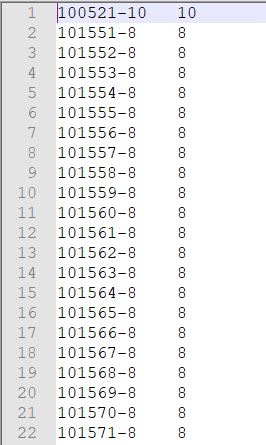
\includegraphics[width=0.4\textwidth]{BayesPredictResult.png}
	\caption{预测结果 \label{fig:BayesPredictResult}}
\end{figure}

\section{Spark实现}
\subsection{简介}
ml和mllib都是Spark中的机器学习库,目前常用的机器学习功能2个库都能满足需求。
spark官方推荐使用ml, 因为ml功能更全面更灵活,未来会主要支持ml,mllib很有可能会被废弃(据说可能是在spark3.0中deprecated)。

两者的不同在于ml主要操作的是DataFrame, 而mllib操作的是RDD,也就是说二者面向的数据集不一样。相比于mllib在RDD提供的基础操作,ml在DataFrame上的抽象级别更高,数据和操作耦合度更低。

DataFrame是Dataset的子集,也就是Dataset[Row], 而DataSet是对RDD的封装,对SQL之类的操作做了很多优化。
相比于mllib在RDD提供的基础操作,ml在DataFrame上的抽象级别更高,数据和操作耦合度更低。
ml中的操作可以使用pipeline, 跟sklearn一样,可以把很多操作(算法/特征提取/特征转换)以管道的形式串起来,然后让数据在这个管道中流动。
ml中无论是什么模型,都提供了统一的算法操作接口,比如模型训练都是fit;不像mllib中不同模型会有各种各样的trainXXX。
mllib在spark2.0之后进入维护状态, 这个状态通常只修复BUG不增加新功能。

所以综上我们在这里使用ml库来实现操作。
\subsection{数据预处理:特征提取}
\subsubsection{计算TF-IDF}
第一步:读取原文本转换成DataFrame

注意:由于Spark2.0起,SQLContext、HiveContext已经不再推荐使用,改以SparkSession代之,故本文中不再使用SQLContext来进行相关的操作,关于SparkSession的可以参看Spark2.0的官方文档。Spark2.0以上版本的spark-shell在启动时会自动创建一个名为spark的SparkSession对象,当需要手工创建时,SparkSession可以由其伴生对象的builder()方法创建出来。RDD转DataFrame的实现通过toDF接口来实现。使用举例如下:


我们的文档是已经经过前面预处理过的文档,每个文件表示一个样本,每个样本名字为“文件名-类名编号”,文件内容由邮件单词构成,每一行为一个单词。

第二步:分词处理

分词使用的是RegexTokenizer库。根据官方文档,RegexTokenizer通过正则化式子来划分句子。在前面的处理中我们已经得到了样本中单词的划分使用的是换行符,所以正则表达式使用的是“$\backslash s$”表示切分符为包括空格、制表符、换页符等空白字符的其中任意一个。使用示例如下:
\begin{lstlisting}[language={Scala},numbers=left,numberstyle=\tiny,%frame=shadowbox,  
  rulesepcolor=\color{red!20!green!20!blue!20},  
  keywordstyle=\color{blue!70!black},  
  commentstyle=\color{blue!90!},  
  basicstyle=\ttfamily]  
val regexTokenizer = new RegexTokenizer()
  .setInputCol("sentence")
  .setOutputCol("words")
  .setPattern("\\s")
\end{lstlisting}\par

第三步:将单词转换成对应的矩阵,计算频率

根据官方文档API,FeatureHasher的作用是将一组分类或数字特征投影到指定尺寸的特征向量中(通常远小于原始特征空间的特征向量)。这是使用散列技巧将要素映射到特征向量中的索引来完成的。

其中特征列每列可能包含数字或字符串列。列数据类型的行为和处理如下:

数字列:对于数字要素,列名称的哈希值用于将要素值映射到要素向量中的索引。
默认情况下,数字要素不被视为字符串列(即使它们是整数)。
要将它们视为字符串列,请使用categoricalCols参数指定相关列。

字符串列:对于字符串,字符串"column\_name = value"的哈希值用于映射到矢量索引,
指示符值为1.0。因此,类别特征是“一热”编码(类似于使用OneHotEncoder)。

布尔列:布尔值的处理方式与字符串列相同。
也就是说,布尔特征表示为“column\_name = true”或“column\_name = false”,
指示符值为1.0。忽略空(缺失)值(在结果特征向量中隐式为零)。

使用举例如下:
\begin{lstlisting}[language={Scala},numbers=left,numberstyle=\tiny,%frame=shadowbox,  
  rulesepcolor=\color{red!20!green!20!blue!20},  
  keywordstyle=\color{blue!70!black},  
  commentstyle=\color{blue!90!},  
  basicstyle=\ttfamily]  
val hasher = new FeatureHasher()
  .setInputCols("real", "bool", "stringNum", "string")
  .setOutputCol("features")
\end{lstlisting}\par

第四步:计算TF-IDF

ml库中的IDF类根据给出的文档计算相应的IDF,IDFModel采用特征向量(通常从HashingTF或CountVectorizer创建)并缩放每个特征。直观地,它降低了在语料库中频繁出现的特征的权重。使用示例如下:
\begin{lstlisting}[language={Scala},numbers=left,numberstyle=\tiny,%frame=shadowbox,  
  rulesepcolor=\color{red!20!green!20!blue!20},  
  keywordstyle=\color{blue!70!black},  
  commentstyle=\color{blue!90!},  
  basicstyle=\ttfamily]  
val idf = new IDF().setInputCol("rawFeatures").setOutputCol("features")
\end{lstlisting}\par

\subsubsection{计算Word2Vec}
Word2Vec 是一种著名的词嵌入(Word Embedding) 方法,它可以计算每个单词在其给定语料库环境下的分布式词向量(Distributed Representation,亦直接被称为词向量)。词向量表示可以在一定程度上刻画每个单词的语义。

如果词的语义相近,它们的词向量在向量空间中也相互接近,这使得词语的向量化建模更加精确,可以改善现有方法并提高鲁棒性。词向量已被证明在许多自然语言处理问题,如:机器翻译,标注问题,实体识别等问题中具有非常重要的作用。

​ Word2vec是一个Estimator,它采用一系列代表文档的词语来训练Word2VecModel。该模型将每个词语映射到一个固定大小的向量。Word2VecModel使用文档中每个词语的平均数来将文档转换为向量,然后这个向量可以作为预测的特征,来计算文档相似度计算等等。

​ Word2Vec具有两种模型,其一是 CBOW ,其思想是通过每个词的上下文窗口词词向量来预测中心词的词向量。其二是 Skip-gram,其思想是通过每个中心词来预测其上下文窗口词,并根据预测结果来修正中心词的词向量。两种方法示意图如下图所示:
\begin{figure}[htbp]
	\centering
	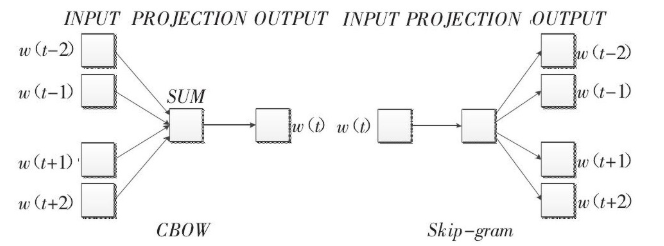
\includegraphics[width=0.6\textwidth]{word2vecModel.png}
	\caption{CBOW和Skip-gram模型 \label{fig:Word2VecModel}}
\end{figure}
总结简单来说,Word2Vector实际上就是用神经网络来实现词向量的生成。
使用举例如下:
\begin{lstlisting}[language={Scala},numbers=left,numberstyle=\tiny,%frame=shadowbox,  
  rulesepcolor=\color{red!20!green!20!blue!20},  
  keywordstyle=\color{blue!70!black},  
  commentstyle=\color{blue!90!},  
  basicstyle=\ttfamily]  
val word2Vec = new Word2Vec().setInputCol("text").
	setOutputCol("features").
	setVectorSize(500).setMinCount(0)
\end{lstlisting}\par

\subsection{朴素贝叶斯}
ml库中的NaiveBayes类实现了朴素贝叶斯模型。支持多项式朴素贝叶斯,可以直接用TF-IDF的结果进行训练,模型可调参数有:特征值列名(featuresCol)、标签列名(labelCol)、模型类型(modelType,默认为多项式朴素贝叶斯)、平滑系数(smoothing)等。使用示例如下:
\begin{lstlisting}[language={Scala},numbers=left,numberstyle=\tiny,%frame=shadowbox,  
  rulesepcolor=\color{red!20!green!20!blue!20},  
  keywordstyle=\color{blue!70!black},  
  commentstyle=\color{blue!90!},  
  basicstyle=\ttfamily]  
val model = new NaiveBayes().setFeaturesCol("features").
	setModelType("multinomial")
\end{lstlisting}\par
\subsection{SVM}

\subsection{结果对比}
使用hadoop的MapReduce多种方法实现出来的准确率如下表所示:
\end{document}
